\documentclass[10pt,letterpaper,bibliography=totoc]{scrartcl}

\usepackage[letterpaper,margin=1.2in]{geometry}
\usepackage{helvet}
\usepackage[utf8]{inputenc}
\usepackage{graphicx}
\usepackage[hyphens]{url}
\usepackage{hyperref}
\usepackage[all]{hypcap} 
\usepackage{xcolor}
\usepackage{listings}
\usepackage[T1]{fontenc}
\usepackage{verbatim}
\usepackage[parfill]{parskip}

\lstset{
    basicstyle=\scriptsize,
    numbers=left,
    numberstyle=\scriptsize,
    stepnumber=1,
    numbersep=5pt,
    showspaces=false,
    showstringspaces=false,
    showtabs=false,
    frame=shadowbox,
    tabsize=4,
    captionpos=b,
    breaklines=true,
    breakatwhitespace=false,
    keywordstyle=\color{blue!70},
    commentstyle=\color{red!50!green!50!blue!50},
    rulesepcolor=\color{red!20!green!20!blue!20},
    numberbychapter=false,
    stringstyle=\ttfamily
}

\setcounter{tocdepth}{2}

\hypersetup{
    colorlinks=true,
    breaklinks=true,
    urlcolor=blue,
    linkcolor=black
}

\begin{document}

\author{Orkun Krand}
\title{Assignment 3}
\subtitle{Fall 2017\\ CS834 Introduction to Information Retrieval\\ Dr. Michael Nelson}
\maketitle
\newpage

\section{Question 6.1}
\subsection {Question}
Using the Wikipedia collection provided at the book website, create a sample of stem clusters by the following process:
\begin{enumerate}
    \item Index the collection without stemming.
    \item Identify the first 1,000 words (in alphabetical order) in the index.
    \item Create stem classes by stemming these 1,000 words and recording which words become the same stem.
    \item Compute association measures (Dice's coefficient) between all pairs of stems in each stem class. Compute co-occurrence at the document level.
    \item Create stem clusters by thresholding the association measure. All terms that are still connected to each other form the clusters.
\end{enumerate}

Compare the stem clusters to the stem classes in terms of size and the quality (in your opinion) of the groupings.

\subsection{Methodology}
\href{https://docs.python.org/2.3/lib/module-cPickle.html}{CPickle} was utilized to speed processes up. I created the \texttt{stem.py} script to define the initial stem classes from the list of 1,000 words.  This list was created using the inverted index I created for assignment 2. Roughly the first 15,000 items in list were/had digits so I used entries between 15,000 and 16,000. I used a threshold of 0.1 to clean up my result. Any stemmed words that exists in each class with a score lower than 0.1 were removed from their class. 

\subsection{Results}
The initial stemming of the 1,000 words produced the following stem classes:

\noindent
aln: aln, alnes\\
alo: aloe, aloes\\
all: alling, all, alles, alle\\
alm: alm, alms\\
alkaloid: alkaloids, alkaloid\\
alight: alight, alighted\\
alkalin: alkaline, alkalinity\\
alexandrin: alexandrines, alexandrine\\
allori: allori, allory\\
alley: alleys, alley\\
alien: alienated, alienate, aliens, alien, alienation, alienates, alienating\\
alpin: alpin, alpines, alpine\\
alexandr: alexandr, alexandre\\
alfr: alfre, alfred, alfr\\
almanac: almanacs, almanac\\
alt: alt, altes, alte\\
allergi: allergies, allergy\\
allig: alligator, alligators\\
altdorf: altdorfer, altdorf\\
alp: alps, alpes, alpe, alp\\
alma: alma, almas\\
allemand: allemandes, allemande\\
allel: alleles, allele\\
allegori: allegories, allegory\\
allo: allo, allos\\
alphabet: alphabetical, alphabetically, alphabet, alphabetized, alphabetic, alphabets\\
altitud: altitude, altitudes\\
algebra: algebraic, algebras, algebraically, algebra\\
alli: allies, allis, alli, allying, allied, ally, allie\\
alfi: alfie, alfy\\
almont: almont, almonte\\
aleutian: aleutians, aleutian\\
almshous: almshouse, almshouses\\
alter: altered, altering, alteration, alterations, alters, alter\\
altern: alternator, alternating, alternators, alternated, alternatively, alternate, alternatives, alternately, alterning, alternative, alternations, alternates\\
alphen: alphen, alphenal\\
almond: almond, almonds\\
alin: aline, alin\\
allyl: allylic, allyl\\
altar: altars, altar\\
algar: algars, algar\\
alexi: alexie, alexi, alexis\\
alloc: allocates, allocation, allocate, allocations, allocated, allocating\\
allstar: allstar, allstars\\
allotrop: allotrope, allotropes\\
allus: allusion, allusions\\
allur: alluring, allure\\
algarv: algarve, algarves\\
almoravid: almoravid, almoravids\\
alleg: allegedly, alleging, allegations, alleged, allegation, alleges, allege\\
allud: allude, alluded, alludes\\
alik: alikes, alike\\
alex: alex, alexs\\
algorithm: algorithmic, algorithms, algorithm\\
almon: almoners, almoner\\
alkyl: alkyl, alkylating\\
alia: alia, alias\\
align: aligning, align, alignable, aligns, aligned, alignments, alignment\\
allround: allround, allrounder\\
alon: alone, alones, alon\\
alor: alor, alors\\
alias: aliasing, aliases\\
alouett: alouettes, alouette\\
allot: allotment, allot, allotted\\
allow: allows, allowing, allow, allowed, allowe, allowances, allowable, allowance\\
alloy: alloy, alloys, alloyed\\
alland: alland, allande\\
alga: alga, algae\\
allianc: alliance, alliances\\
allevi: alleviating, alleviate\\
alfieri: alfieri, alfieris\\

The following is the stem classes produced when I introduced Dice's coefficient into the mix. I tested the code with two different thresholds (0.1 and 0.0001) to confirm that the threshold was working. As expected, the lower threshold, included more stems and words. Qualitywise, the following classes seem more refined compared to the initial results since it only includes strongly linked words. 
\noindent
0.1 Results\\
almoravid: almoravid, almoravids\\
alloc: allocation, allocating, allocate, allocations\\
allotrop: allotrope, allotropes\\
almon: almoners, almoner\\
algorithm: algorithmic, algorithms, algorithm\\
algebra: algebraic, algebraically\\
align: aligning, alignable\\
alkaloid: alkaloids, alkaloid\\
alexandrin: alexandrines, alexandrine\\
alleg: allegation, alleges, alleged, allegedly\\
aleutian: aleutians, aleutian\\
allow: allowances, allows, allow, allowance\\
almshous: almshouse, almshouses\\
alter: alterations, alteration\\
allot: allotment, allotted\\

0.00001 Results\\
altern: alternating, alternator, alternatively, alternate, alternatives, alternative\\
almoravid: almoravid, almoravids\\
alloc: allocation, allocating, allocate, allocations\\
allotrop: allotrope, allotropes\\
almon: almoners, almoner\\
algorithm: algorithmic, algorithms, algorithm\\
algebra: algebraic, algebraically, algebra\\
alphabet: alphabet, alphabetical\\
altitud: altitude, altitudes\\
alkaloid: alkaloids, alkaloid\\
alexandrin: alexandrines, alexandrine\\
alleg: allegedly, allegations, alleged, allegation, alleges, allege\\
alli: allied, allies, ally\\
allianc: alliance, alliances\\
alien: alien, aliens\\
align: aligning, alignable\\
aleutian: aleutians, aleutian\\
allow: allows, allowing, allow, allowed, allowe, allowances, allowance\\
almshous: almshouse, almshouses\\
alter: alterations, alteration\\
allot: allotment, allotted\\

\section{Question 6.2}
\subsection {Question}
Create a simple spelling corrector based on the noisy channel model. Use a single-word language model, and an error model where all errors with the same edit distance have the same probability. Only consider edit distances of 1 or 2. Implement your own edit distance calculator (example code can easily be found on the Web)

\subsection{Methodology}
The spelling corrector will be based on \href{http://norvig.com/spell-correct.html}{Peter Norvig's corrector} he wrote while traveling on a plane. For the sample text I used \href{http://norvig.com/big.txt}{big.txt} which I found on Peter Norvig's website. The probability of a word is calculated with the following formula:

\[P(w) = \frac{Count_w}{N}\]

where \(Count_w\) is the word count for word \(w\) and \(N\) is the sum of all word counts.\\

In order to determine if a word is right or wrong, I found all the words with edit distance one and two to each word. Assuming the correct word will be the one with shorter edit distance, those words with a shorter edit distance and higher probability are picked as the correct word. 

The code can be found in \texttt{spell.py}.

\subsection{Results}
Here is a screenshot of a couple words I tested. If it can't come up with a replacement ``correct'' word, the script returns the original word.
\begin{figure}[h!]
\centering
\label{fig:sample_spelling}
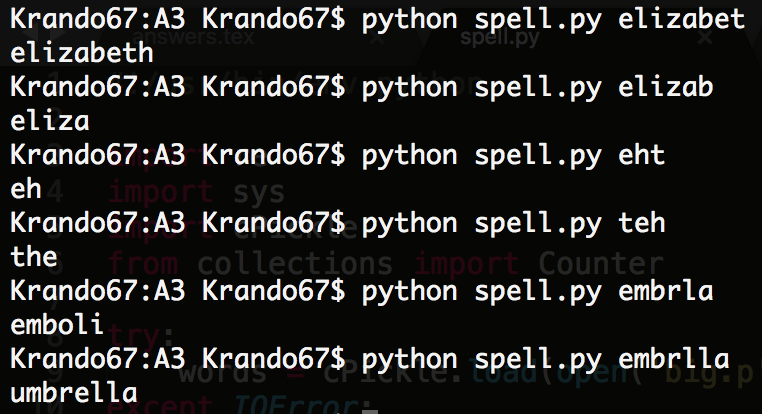
\includegraphics[scale=.5]{sample_spelling.png}
\caption{Sample Spelling Correcter Output}
\end{figure}


\section{Question 6.5}

\subsection{Question}
Describe the snippet generation algorithm in Galago. Would this algorithm
work well for pages with little text content? Describe in detail how you would
modify the algorithm to improve it.

\subsection{Answer}
The main idea of the snippet generator is that it looks for the query words in the text of the document. Once a match is found, the generator grabs the 5 words before and after to create a snippet region. It can handle overlaps in snippet regions. This search goes on until the character threshold is reached at which point the generator stops going through the document. Snippet's ready. 

This algorithm would fail to create a useful snippet for a page with little text content since it relies on document text to generate the snippet regions. If there are no words in the document, then the generator has nothing to compare the query words to.

Taking into account the query word density is probably a good idea as it would improve the results shown. So for example if a user is searching for the phrase ``tropical fish'', and the snippet generator finds the word tropical over and over again, that would be enough to generate a snippet. This will force the algorithm to run for longer, increasing overhead but maybe we would be using Galago today instead of \href{www.google.com}{Google} if they cared to implement it. In order to implement this, snippet regions could be entered into a hash table which keeps track of which query words are in which snippet regions. Afterwards, the hash table would be analyzed to find which snippet regions have the highest density of query words. Those snippet regions would be concatenated to create the final snippet.

\section{Question 6.9}
\subsection {Question}
Give five examples of web page translation that you think is poor. Why do you think the translation failed?

\subsection{Methodology}
I will use the \href{https://safari-extensions.apple.com/details/?id=com.sidetree.Translate-S64NDGV2C5}{Translate extension of Apple's Safari} (I don't normally use Safari but Chrome knows me too well) which uses Google or Bing to translate 3 pages from Turkish to English and two pages from English to Turkish. 

\subsection{Examples}
\subsubsection{\href{http://www.motosikletdergisi.com/haber/436/motosiklet-satislari-dususte.html}{Motosiklet satışları düşüşte}}
This is a news article about the low number of motorcycle sales in Turkey. While the translation is readable, it is very hard to understand. Some words are not translated at all. The first paragraph was going well until the last sentence where the translator butchered it quite bad. This was caused by a word that has more than one meaning translated as one meaning when it should be translated as the other meaning. In this specific example, the word ``adet'' means each or copies. ``Average 140 thousand copies'' makes no sense since motorcycles aren't made out of paper. Ommitting the culprit would've probably solved the problem since in English, we don't have to say ``140 thousand each motorcycle''. 

Also it translates the currency from Turkish Lira to British Pounds without changing the number. Considering the value difference between the two currencies, someone reading this will think Turkish people pay \$4,500 per year for motorcycle insurance when the actual number is \$900.

\subsubsection{\href{https://www.sahibinden.com/ilan/vasita-otomobil-opel-dizeller-dizeli-dizeleri-dizdi-359464489/detay}{DİZELLER DİZELİ DİZELERİ DİZDİ}}
``Sahibinden'' is a platform for people to sell vehicles, houses, find jobs and so forth. It's very similar to craigslist but it has a better interface. This ad is for a Opel Astra 1.3 diesel car. I will include screenshots in case the ad disappears. 
\begin{figure}[h!]
\centering
\label{fig:car_ad_turkish}
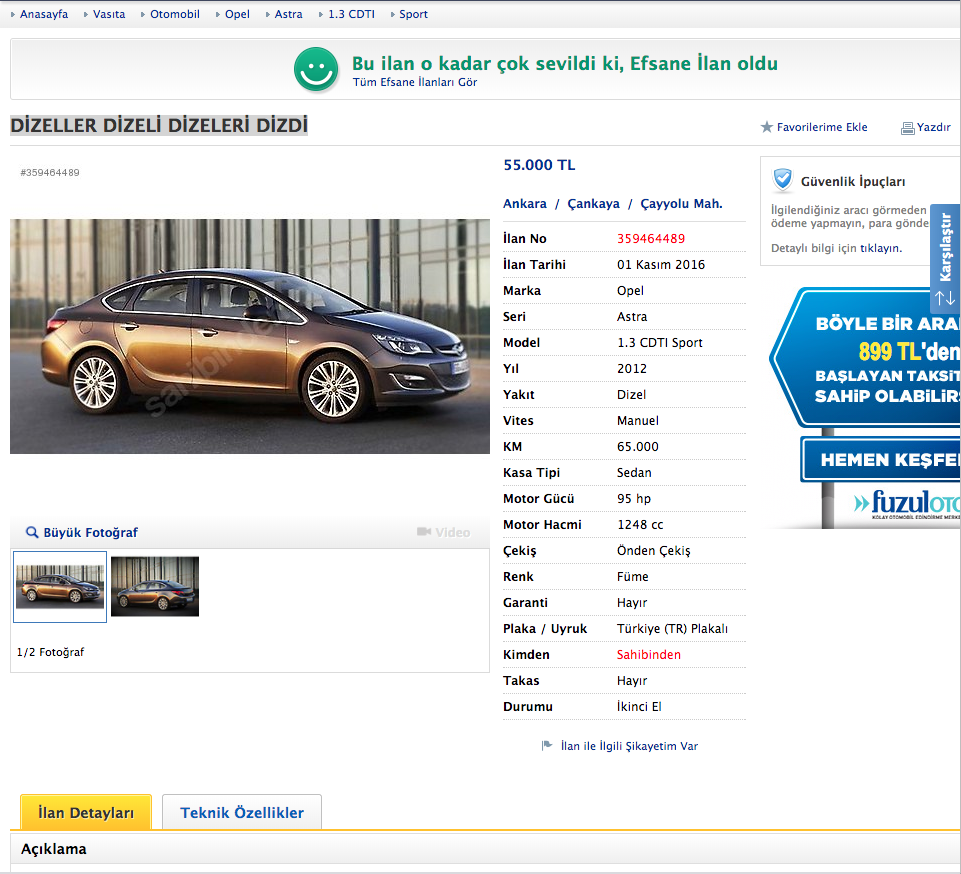
\includegraphics[scale=.5]{opel_turkish.png}
\caption{Opel Astra Turkish}
\end{figure}
\begin{figure}[h!]
\centering
\label{fig:car_ad_english}
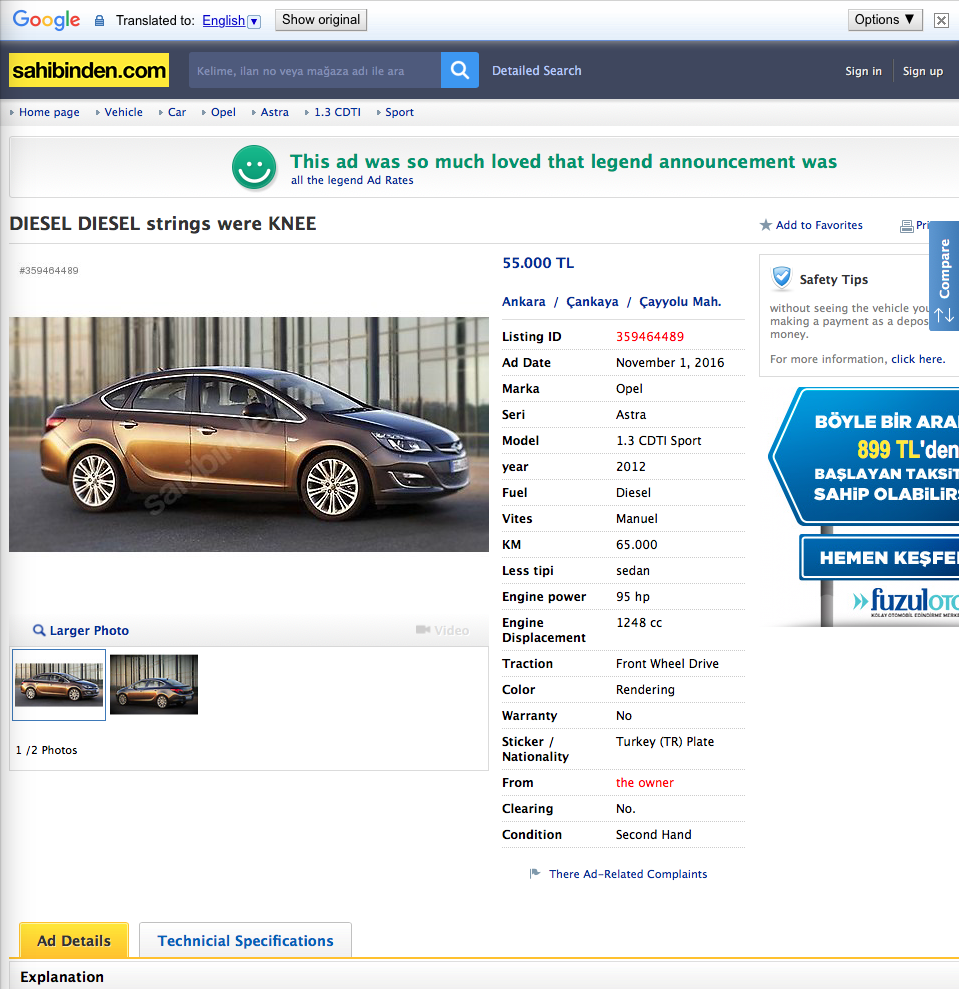
\includegraphics[scale=.5]{opel_english.png}
\caption{Opel Astra English}
\end{figure}

Looking at the information about the vehicle, you will notice that some things don't make any sense, like the color of the vehicle for example. The word they use in the original page ``füme'' translates to smoked but is usually referred to the color you see in the picture. After checking out various dictionaries, I have no idea how they came up with the word ``rendering''. 

\begin{figure}[h!]
\centering
\label{fig:poem_english}
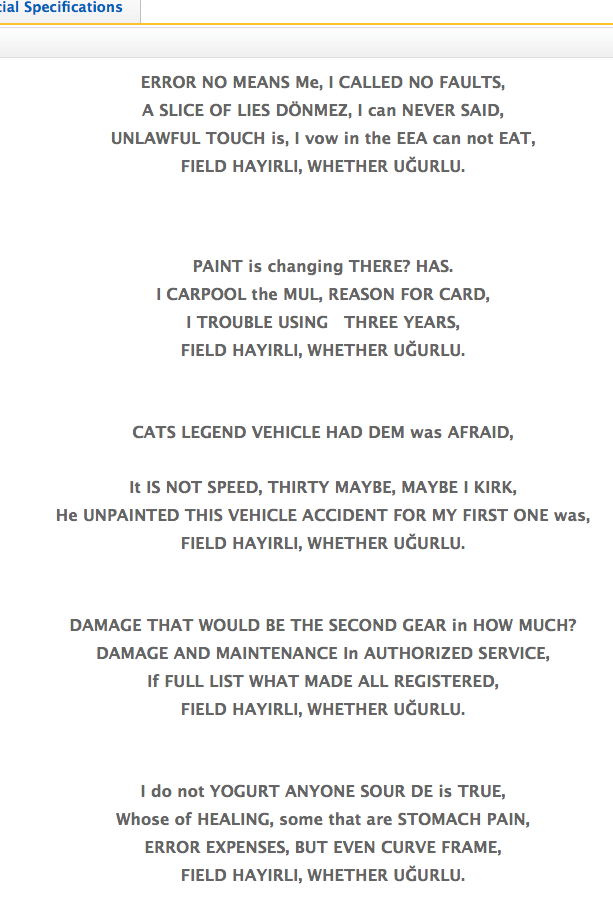
\includegraphics[scale=.5]{poem_english.png}
\caption{Car Ad Poem English}
\end{figure}
\begin{figure}[h!]
\centering
\label{fig:poem_turkish}
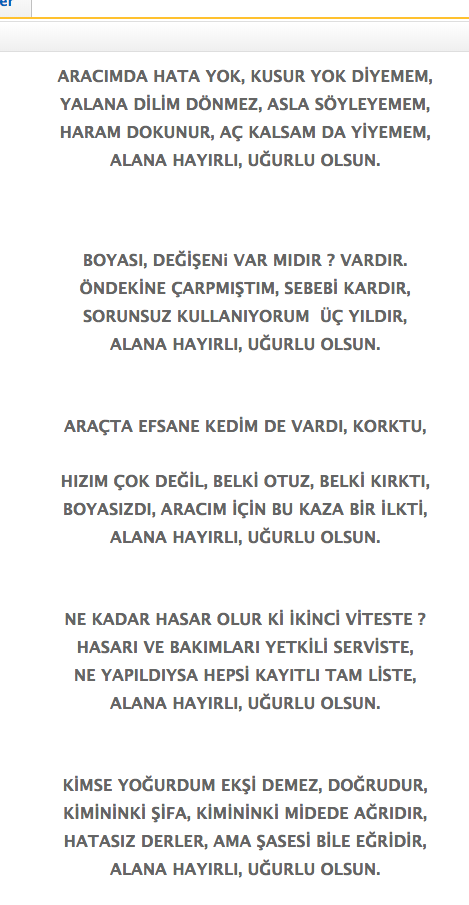
\includegraphics[scale=.5]{poem_turkish.png}
\caption{Car Ad Poem Turkish}
\end{figure}
The best part of this ad is the description. The person who posted this ad decided to write a poem that describes his/her vehicle. I will let you try to make some sense of it. The main reason translation fails so bad is because the poem isn't really written in a traditional sentence structure. It puts words in different orders to ensure it rhymes but this breaks the translator as I assume it looks at the previous and next word (or the whole sentence) when picking a translation for each word. 

\subsubsection{\href{http://www.hurriyet.com.tr/lamborghiniden-butce-dostu-arac-mi-geliyor-40346732}{Lamborghini'den bütçe dostu araç mı geliyor?}}
This is a news article from a mainstream newspaper website (the first one was a motorcycle magazine's website). This review is mostly bad because the algorithm is not good enough. It is a news article so it's properly written (no spelling mistakes, well structured sentences). The translator just fails to recognize some words such as the word ``demek'' in the first sentence. It means to say something in English. It can also be thought of as calling something. So if we were to put the word at the very beginning of the sentence, that would make the first sentence perfect. It's mostly small things like this that ruin the translation on this page. 

\subsubsection{\href{https://www.autotrader.com/car-news/here-are-some-tips-for-parting-with-a-car-you-love-270569}{Here Are Some Tips for Parting With a Car You Love}}
Similar to the problems with translating from Turkish to English, Bing's English to Turkish translator has issues. The first sentence of the second paragraph doesn't make much sense. We can guess that he probably owned it for 2 years. But the bigram ``daily driver'' is a unique because the word ``driver'' generally means someone that drives a vehicle. The translator seems to have an easier time with every day words compared to words like ``bolstered'' which nobody uses daily. When a sentence has more common words, it seems to be able to process more words at a time (bigrams for uncommon words vs. five-gram for more common words). 

\subsubsection{\href{https://en.wikipedia.org/wiki/Norfolk,_Virginia}{Norfolk, Virginia}}
I thought the translation of Wikipedia pages would be the worst which is why I saved it for last but this is a surprisingly good translation. I was able to observe how well the translator works from the previous examples but this is better compared to others. Maybe Google's better at translating from English than translationg to English. But the main reason it's better in my opinion is because the Wikipedia page contains a lot of special names such as ``Chesapeake'', or ``Norfolk Southern Railway''. These help the reader understand the context even if other words fail to translate correctly.

\subsection{Discussion}
The first two pages were translated from Turkish to English using Google Translate. The next two were translated using Bing and the last one was translated using Google as well. The translator seems to get confused by words that have more than one meanings. Poems definitely throw it off and provide a lower accuracy translation. Sentences that give data are better translated. The ones with numerical data are even better since the languages have pretty well defined rules as to what comes before or after numbers. 

\section{Question MLN2}
\subsection{Question}
Using the small wikipedia example, choose 10 words and compute MIM, EMIM, chi square, dice association measures for full document \& 5 word windows (cf. pp. 203-205)

\subsection{Methodology}
I created \texttt{mln2.py} which tackles this problem. It uses the same inverted index as \texttt{6.1} to calculate the measures requested. 
The words I picked were:\\
\begin{itemize}
    \item umbrella
    \item messenger
    \item cramps
    \item equestrian
    \item sea
    \item everlasting
    \item association
    \item vehicle
    \item python
    \item motorcycle
\end{itemize}

\subsection{Results}
The words ``python'' and ``everlasting'' returned the same results for each type of association. X2 and Dice seem to be better compared to MIM and EMIM as they return related words. Dice performed better than X2 especially for the word ``sea''. For that word, Dice was spot on, suggesting very related terms like island, ocean, ships, etc. Worst seems to be EMIM as it kept suggesting the same 8 words for the words ``association'', ``vehicle'', and ``motorcycle''. None of those 8 words were related to the query word. 

\noindent
umbrella\\
  MIM  ['tumen', 'haoma', 'hyperdrive', 'spaceships', '1521ad', 'tuuli', 'b0007bfxk4', 'vedism', 'vorgejz', 'temp07']\\
  EMIM ['which', '1', '2008', '4', 'on', 'categories', 'offline', 'gnu', '7ecommon', '501']\\
  X2   ['tumen', 'haoma', 'hyperdrive', 'spaceships', '1521ad', 'tuuli', 'b0007bfxk4', 'vedism', 'vorgejz', 'temp07']\\
  Dice ['confucianism', 'amendment', 'token', 'undesirable', 'disagreed', 'hostages', 'salvadoran', 'solemn', 'repel', 'unconstitutional']\\\\
messenger\\
  MIM  ['kouga', 'wftv1', 'susans', 'wflc', 'furry', 'wkhk', 'casbah', 'brookmeade', 'orseno', 'wedekind']\\
  EMIM ['2008', '2', 'on', 'categories', 'offline', 'gnu', '7ecommon', '501', 's', 'fixalpha']\\
  X2   ['salama', 'wcau', 'kouga', 'wftv1', 'susans', 'wflc', 'furry', 'wkhk', 'casbah', 'brookmeade']\\
  Dice ['salama', 'wcau', 'copious', 'striver', 'personality', 'cared', 'jarvis', 'sanford', 'cochran', 'prophet']\\\\
cramps\\
  MIM  ['gastroenterology', 'boulardii', 'hydrophila', 'frailty', 'challis', 'earshot', 'mismanaged', 'antimotility', 'paregoric', 'mongering']\\
  EMIM ['unhygienic', 'buying', 'drinking', 'eating', 'bed', 'sullivan', 'blood', 'selling', 'getting', 'scale']\\
  X2   ['unhygienic', 'gastroenterology', 'boulardii', 'hydrophila', 'frailty', 'challis', 'earshot', 'mismanaged', 'antimotility', 'paregoric']\\
  Dice ['unhygienic', 'gastroenterology', 'boulardii', 'hydrophila', 'frailty', 'challis', 'earshot', 'mismanaged', 'antimotility', 'paregoric']\\
equestrian\\
  MIM  ['deligia', 'pimplo', 'irredento', 'liamodwyer13', 'louisay', 'corporacy', 'damiano', 'ongarato', 'morbidelli', 'maccabean']\\
  EMIM ['olympics', 'summer', '2008', 'bronze', 'on', 'categories', 'offline', 'gnu', '7ecommon', '501']\\
  X2   ['equestrianism', 'equestrians', 'deligia', 'pimplo', 'irredento', 'liamodwyer13', 'louisay', 'corporacy', 'damiano', 'ongarato']\\
  Dice ['equestrianism', 'equestrians', 'archery', 'fencing', 'deligia', 'pimplo', 'irredento', 'liamodwyer13', 'louisay', 'corporacy']\\\\
sea\\
  MIM  ['kalecik', 'vologda', 'immunities', 'rbeas', 'hoogenboom', 'antillaise', 'krais', 'wheatear', 'balade']\\
  EMIM ['categories', 'offline', 'gnu', '7ecommon', '501', 's', 'fixalpha', '7emonobook', 'cdata', 'disclaimers']\\
  X2   ['2', '4', '5', 'a', 'showtoctoggle', 'tocshowtext', 'tochidetext', '8', 'show', '6']\\
  Dice ['ocean', 'h', 'over', 'island', 'earlier', 'little', 'atlantic', 'ship', 'bay', 'islands']\\\\
everlasting\\
  MIM  ['andy120', 'didactohedron', 'prostration', 'auricular', 'oris', 'admonish', 'starets', 'martyrion', 'deinde', 'divulges']\\
  EMIM ['andy120', 'didactohedron', 'prostration', 'auricular', 'oris', 'admonish', 'starets', 'martyrion', 'deinde', 'divulges']\\
  X2   ['andy120', 'didactohedron', 'prostration', 'auricular', 'oris', 'admonish', 'starets', 'martyrion', 'deinde', 'divulges']\\
  Dice ['andy120', 'didactohedron', 'prostration', 'auricular', 'oris', 'admonish', 'starets', 'martyrion', 'deinde', 'divulges']\\\\
association\\
  MIM  ['pskalka', 'fundation', 'vann', 'kovaciny', 'tcbr', 'immunities', 'landrover4', 'hoogenboom', 'sunbeams', 'kids']\\
  EMIM ['offline', 'gnu', '7ecommon', '501', 's', 'fixalpha', '7emonobook', 'cdata', 'disclaimers', 'mediawiki']\\
  X2   ['national', 'show', 'showtoctoggle', 'tocshowtext', 'tochidetext', '4', '1', '2', '5', '6']\\
  Dice ['national', 'school', 'year', 'retrieved', '2002', '2000', 'team', 'non', 'showtoctoggle', 'tocshowtext']\\\\
vehicle\\
  MIM  ['rbeas', 'numerao', 'skatelikekemp', 'mklimstra', 'skyblue27', 'nichiyoubi', 'samokhodno', 'syx', 'kcci', 'conductive']\\
  EMIM ['on', 'offline', 'gnu', '7ecommon', '501', 's', 'fixalpha', '7emonobook', 'cdata', 'disclaimers']\\
  X2   ['vehicles', 'wheels', 'axle', 'motor', 'cars', 'engine', 'policemen', 'sfoskett', 'tracked', 'tanks']\\
  Dice ['vehicles', 'motor', 'cars', 'wheels', 'engine', 'driving', 'mounted', 'car', 'fitted', 'electronic']\\\\
python\\
  MIM  ['kudrimalai', 'drypetes', 'elephas', 'trijuga', 'disopyros', 'manilkara', 'modesta', 'wcmc', 'shrew', 'dendrocygna']\\
  EMIM ['kudrimalai', 'drypetes', 'elephas', 'trijuga', 'disopyros', 'manilkara', 'modesta', 'wcmc', 'shrew', 'dendrocygna']\\
  X2   ['kudrimalai', 'drypetes', 'elephas', 'trijuga', 'disopyros', 'manilkara', 'modesta', 'wcmc', 'shrew', 'dendrocygna']\\
  Dice ['kudrimalai', 'drypetes', 'elephas', 'trijuga', 'disopyros', 'manilkara', 'modesta', 'wcmc', 'shrew', 'dendrocygna']\\\\
motorcycle\\
  MIM  ['dnq', 'smackdown', 'jugulator', 'indyahh', 'seasalt', 'y2kcrazyjoker', 'derbi', 'toshihisa', 'downeyocean', 'puniet']\\
  EMIM ['categories', 'offline', 'gnu', '7ecommon', '501', 's', 'fixalpha', '7emonobook', 'cdata', 'disclaimers']\\
  X2   ['motogp', 'puniet', 'guintoli', 'capirossi', 'gibernau', '125cc', 'loris', 'dovizioso', 'melandri']\\
  Dice ['motogp', 'brianhe', 'fabrizio', 'cc', 'puniet', 'guintoli', 'capirossi', 'gibernau', '125cc', 'loris']\\

\clearpage
% \begin{thebibliography}{9}
% \bibitem{classtext}
%     Croft, William Bruce, et al. \textit{Search Engines: Information Retrieval in Practice}. Pearson, 2010.
% \end{thebibliography}
\end{document}